\section{Linear Flow matching performs fairly well on periodic datasets}

\subsection{Results}

\subsubsection{$\theta$ flow matching and $x$ flow matching}

Theta flow matching with path integral on $\theta$ works well for non-periodic datasets (see previous notes), but fails on periodic datasets (see previous notes). This is reasonable because the theta path-integral method requires integration over the parameter $\theta$. In a periodic dataset, the representations of $\theta$ and $\theta+T$ are the same. However, integrating from $\theta$ to $\theta+T$ can accumulate errors along the path, producing a non-zero distance even though the two points should be equivalent.

One way to avoid path integration over $\theta$ is to perform path integration over the flow-matching time parameter $t$. Given a dataset containing data points $x$, flow matching learns a velocity field $v(x_t, t)$. This velocity field generates samples by integrating over time, that is, by solving an ODE. Similarly, there is another equation that allows us to compute the log likelihood by integrating over $t$, where $p_0(x_0)$ is the known likelihood of the source distribution.
\[
\log p_1(x_1)
=
\log p_0(x_0)
-
\int_0^1
\nabla_x \cdot v(x_t, t)\, dt,
\qquad
\frac{dx_t}{dt} = v(x_t, t),
\]
where $(x_t)_{t\in[0,1]}$ is the trajectory obtained by integrating the ODE (for example, from the source sample $x_0$ to the endpoint $x_1$ in the generative direction used by the model).

In the context of this paper, given a dataset $(x,\theta)$, there are two ways to fit a flow-matching model.

First, we can use $\theta$ as the target and $x$ as the condition:
\[
\frac{d\theta}{dt} = v(\theta_t, t; x).
\]
This is the same setup used in the theta-integral method. Once the velocity field is learned, we can integrate over $t$, to obtain $\log p(\theta \mid x)$. This allows us to compute the log-likelihood ratio and, eventually, the Hellinger distance.

Alternatively, we can use $x$ as the target and $\theta$ as the condition. The advantage of this approach is that it directly learns $\log p(x \mid \theta)$. In neuroscience, $p(x \mid \theta)$ is often single-peaked which is easier to learn. In contrast, for periodic data, $p(\theta \mid x)$ has multiple modes. The disadvantage is that $x$ is high-dimensional, potentially cousing stability issues. Furthermore, computing the the divergence of the high-dimensional velocity field is expensive.

\subsubsection{Gaussian baseline}

In addition to flow matching, we also considered a Gaussian baseline. This method discretizes $\theta$ into bins and estimates the mean response within each bin. Given the mean $\mu$, we compute the residuals $x-\mu$ and concatenate the residual vectors across all bins to estimate a single covariance matrix that is invariant to $\theta$. Thus, each $p(x \mid \theta)$ is modeled as a Gaussian distribution with a diagonal, constant covariance matrix. Under this model, the Hellinger distance can be computed analytically (see Methods).

\subsubsection{$\theta$ flow matching and $x$ flow matching do not perform well on high-dimensional periodic datasets, Gaussian baseline performs well}

Both the theta-flow and x-flow methods perform well on non-periodic data, but fail on periodic data, unless the data dimensionality is very low, for example, 3D data (which is not shown in this note). I also checked the posterior estimates. In the periodic case, the theta-flow method learns only one mode instead of multiple modes (not shown). Overall, theta-flow and x-flow methods are better than the previous theta integral on theta space method because they works on low-dimensional periodic data (not shown), however, they still fail on high-dimensional periodic data.

Interestingly, the simple binning-based diagonal Gaussian method estimates the Hellinger distance reasonably well for both non-periodic and periodic data.

\subsubsection{Linear flow matching performs well}

These results motivates a hypothesis: If a method is too flexible, i.e., makes few assumptions, it performs well only when there is sufficient data. In contrast, if a method is less flexible but incorporates reasonable assumptions, such as Gaussianity, it can perform well with limited data, although it may not reach perfect performance.

Motivated by this hypothesis, we constructed a linear flow-matching method that imposes stronger assumptions on the velocity field. In standard flow matching, the velocity is modeled by a neural network,
\[
v_\phi(x, t; \theta).
\]
Here, we impose the stronger assumption that the velocity field is linear:
\[
v = A x + b(\theta),
\]
where $b(\theta)$ is a neural network and $A$ is a learnable matrix. We can further impose different structures on $A$ to control the strength of the constraint. For example, $A$ can be a scalar, a diagonal matrix, a diagonal matrix whose entries depend on $\theta$, or a low-rank matrix.

As long as $v$ is a linear function of $x$, the analytical solution shows that the target distribution is Gaussian (see Methods). Therefore, the linear flow-matching method approximates the target distribution as a Gaussian distribution with different possible covariance structures.

We applied this family of linear flow-matching methods to the non-periodic dataset and found that they perform well, although not perfectly, because the target distribution is not exactly Gaussian. For the periodic dataset, unlike the assumption-free x-flow method, linear flow matching can recover the periodic structure. Its performance is comparable to that of the classifier-decoding method (see Figures~\ref{fig:linear-fm-composite-1} and~\ref{fig:linear-fm-composite-2}).

\begin{figure}[!htbp]
  \centering
  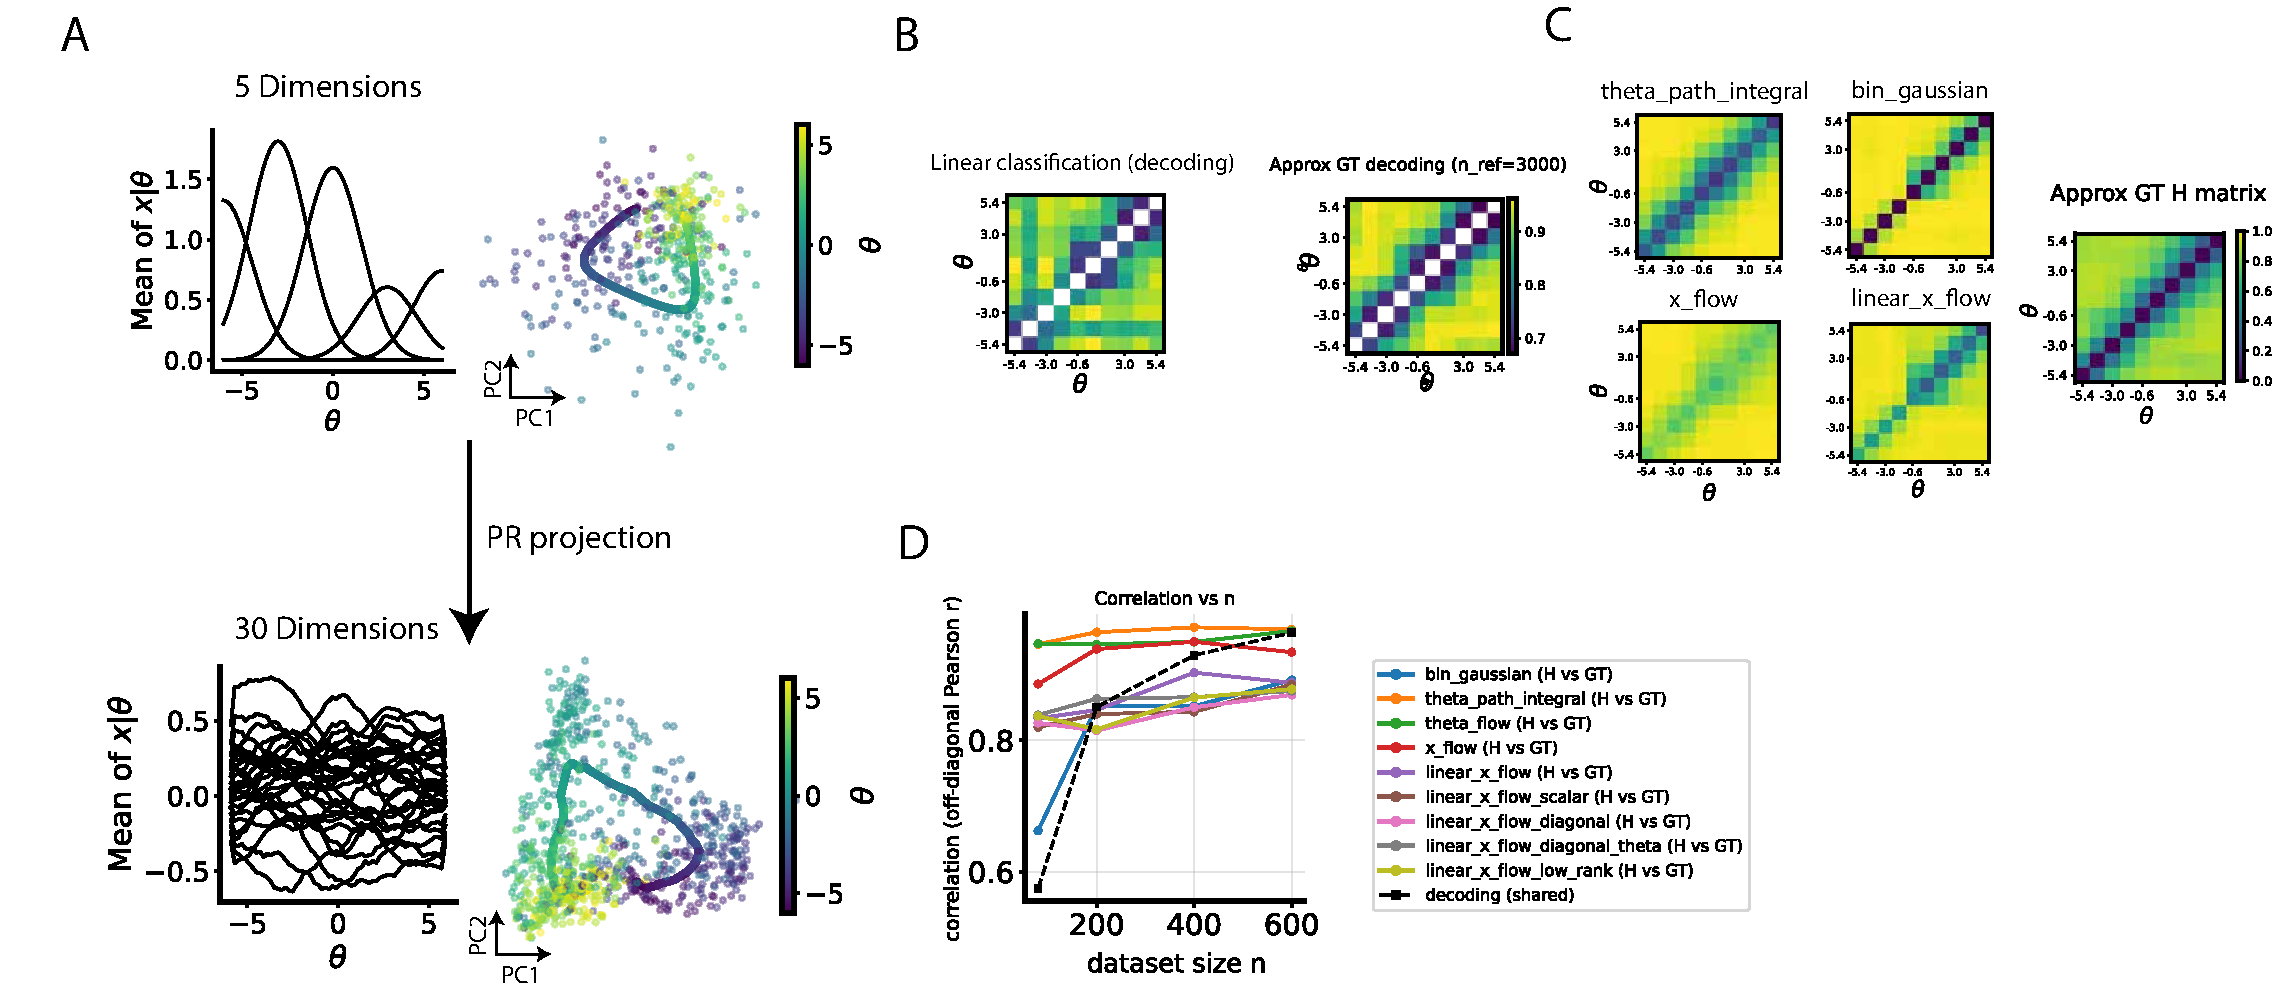
\includegraphics[width=\linewidth]{notes/figures/2026-04-30-linear-flow-matching/linear_flow_matching_fig2.pdf}
  \caption{%
  Flow matching methods and gaussian baseline methods perform well on non-periodic datasets.
  (A) Mean response curves and PCA embeddings before/after PR projection. Data are generated from 5D latent space then projected to high-dimensional space for feeding to different methods estimating RDM. For the PCA visualization, we computed the binning mean of the data first then fitting first PCs for visualization. Scattering points are data projected onto the same PC space.
  (B) We splitted data into bins and for each binned trained a logistic classifier to compute the classification accuracy. Estimated matrix was computed by a n = 200 dataset; while GT was computed by a n = 3000 dataset.
  (C) Estimated Hellinger-distance matrices for several estimators versus an approximate ground-truth $H$ matrix. GT $H$-matrix was estimated by MC sampling with analytical log likelihood expression in the latent 5D space. Full $n$-sweeps appear in Supplementary Figures~\ref{fig:linear-fm-si-1} and~\ref{fig:linear-fm-si-2}.
  (D) Off-diagonal Pearson correlation to that reference as a function of dataset size $n$.
  }
  \label{fig:linear-fm-composite-2}
\end{figure}

\FloatBarrier
\begin{figure}[!htbp]
  \centering
  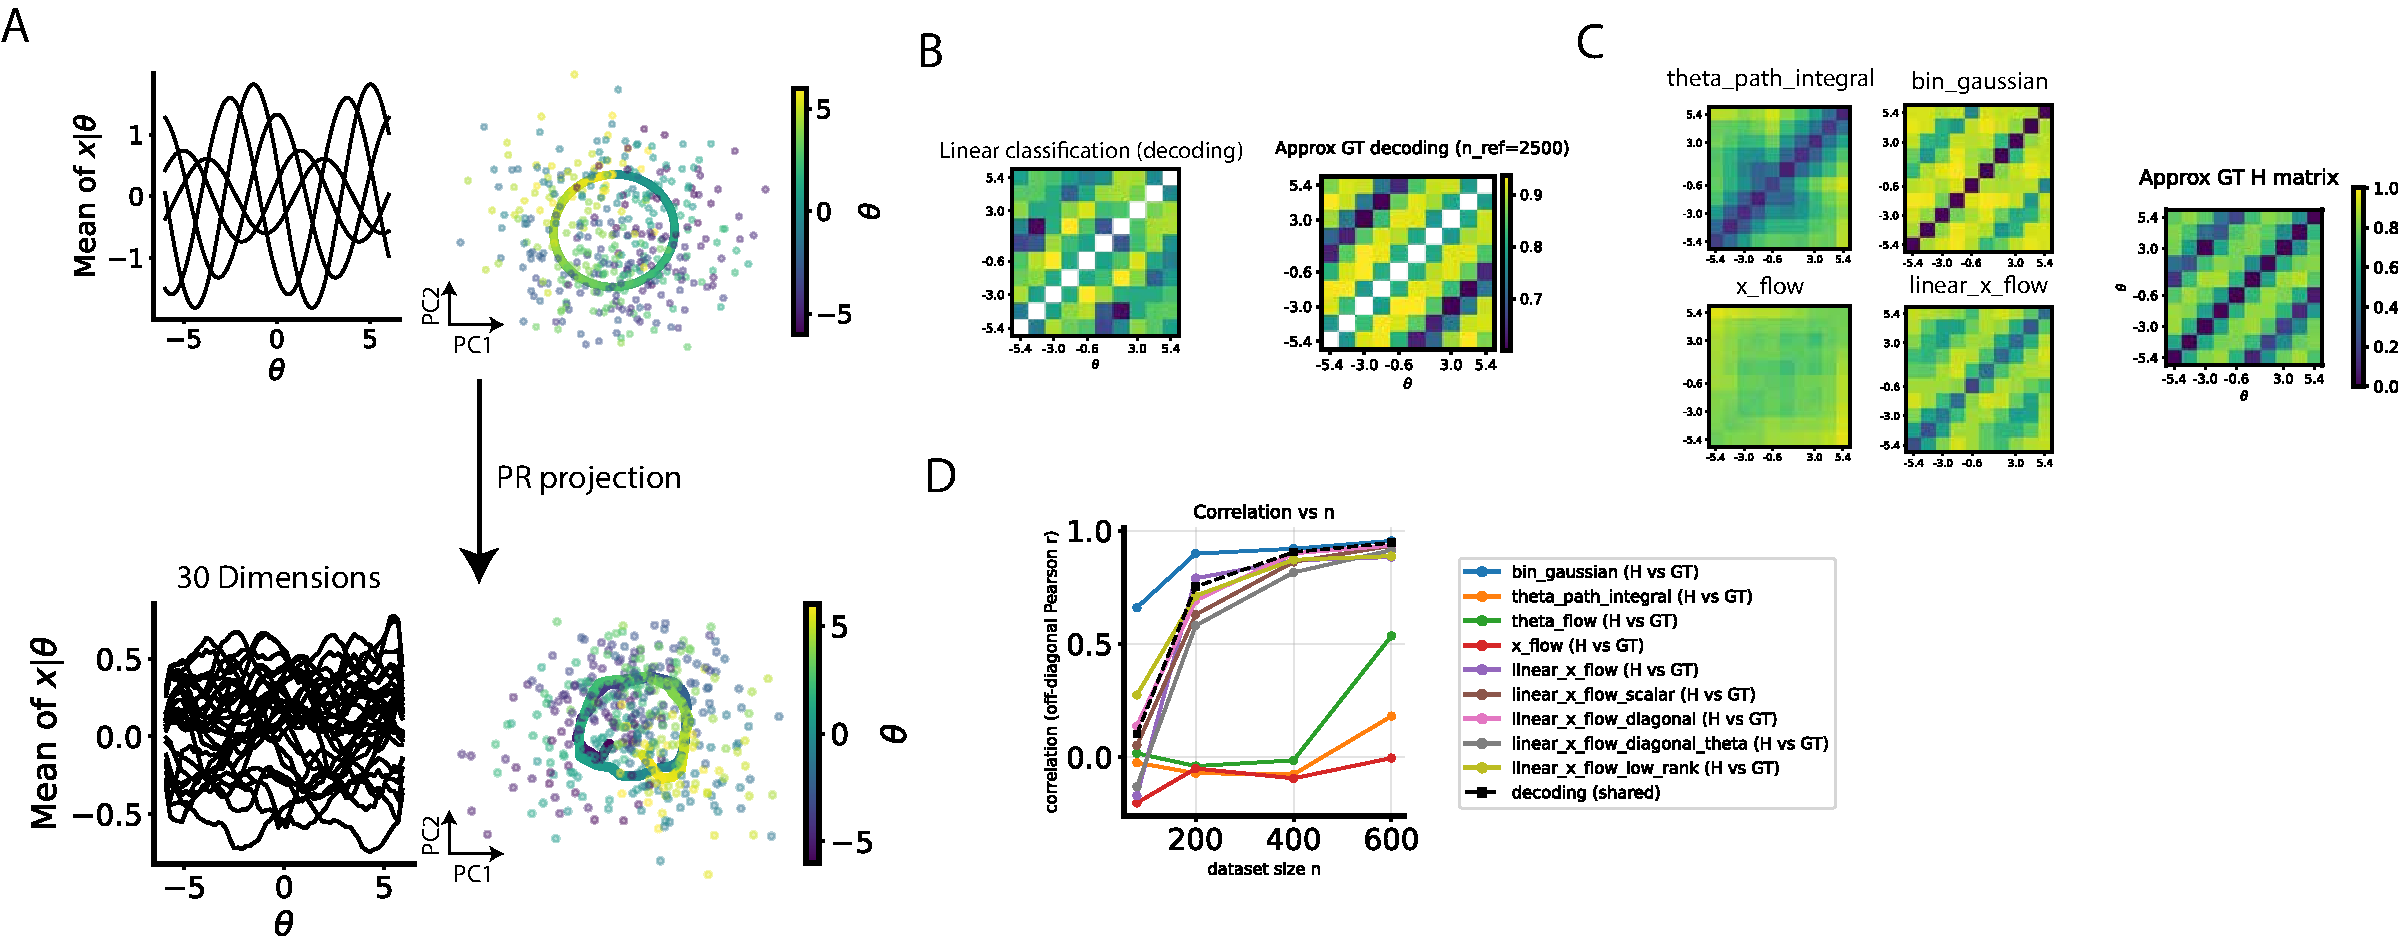
\includegraphics[width=\linewidth]{notes/figures/2026-04-30-linear-flow-matching/linear_flow_matching_fig1.pdf}
  \caption{
    Same as Figure~\ref{fig:linear-fm-composite-2} but for periodic datasets. Linear flow matching and Gaussian baseline methods perform well on periodic datasets. But other flow matching methods fail on high-dimensional periodic datasets.
  }
  \label{fig:linear-fm-composite-1}
\end{figure}


\subsection{Discussion}

Overall, there are several interesting future directions. I list three below.

First, we could develop a more flexible flow-matching method. Linear flow matching is highly constrained because it models the distribution as Gaussian. A possible extension is to add a nonlinear perturbation term to the velocity field, making the model slightly nonlinear and more flexible. Ideally, this method would remain robust while gaining additional expressive power.

Second, we could make the dataset more challenging. The current datasets are relatively simple, so even the binning-based Gaussian method performs fairly well. One possible direction is to make $\theta$ two-dimensional.

Third, we could incorporate dimensionality reduction. Flow matching is very flexible and can easily find shortcuts. If we first constrain the dimensionality of the data, this would effectively make the data denser and may force the model performance to be better constrained by the available data.

\subsection{Methods}

\subsubsection{Non-periodic and periodic datasets}

\paragraph{Non-periodic (Gaussian bumps).}
The non-periodic experiments use the same random-amplitude Gaussian-bump conditional model as in the flow-matching toy note: a scalar stimulus $\theta$ on a bounded interval (no wrapping), paired with a multivariate observation $x\in\mathbb{R}^{d}$.
Stimuli are drawn independently from a uniform density,
\begin{equation}
  \label{eq:theta-uniform-synth}
  \theta \sim \mathrm{Uniform}(\theta_{\mathrm{low}}, \theta_{\mathrm{high}}).
\end{equation}
For each coordinate $j\in\{1,\ldots,d\}$ we fix a tuning center $\theta_j$ by placing $d$ equally spaced points on $[\theta_{\mathrm{low}}, \theta_{\mathrm{high}}]$ (endpoints included).

Before drawing joint samples $(\theta,x)$, we sample one amplitude per coordinate,
\begin{equation}
  a_j \sim \mathrm{Uniform}(a_{\mathrm{low}}, a_{\mathrm{high}}),
  \qquad j = 1,\ldots,d,
\end{equation}
independently across $j$; the vector $(a_1,\ldots,a_d)$ is then held fixed across the dataset.
Given $\theta$, the conditional mean of $x_j$ is a Gaussian bump in $\theta$ centered at $\theta_j$,
\begin{equation}
  \mu_j(\theta) = a_j \exp\!\bigl(-\kappa\,\bigl(\omega\,(\theta - \theta_j)\bigr)^2\bigr),
  \qquad j = 1,\ldots,d,
\end{equation}
with bump precision $\kappa\ge 0$ and stimulus-axis scale $\omega$, and $\mu(\theta)=(\mu_1(\theta),\ldots,\mu_d(\theta))^{\mathsf{T}}$.

Conditionally on $\theta$, the observation is multivariate Gaussian with diagonal covariance.
The generator fixes per-coordinate baseline scales $\sigma_{\mathrm{base},1},\ldots,\sigma_{\mathrm{base},d}$ (linearly spaced between recipe endpoints $\sigma_{x,1}$ and $\sigma_{x,2}$) and per-coordinate activity weights $\alpha_1,\ldots,\alpha_d$.
Under the default additive law (activity enters additively rather than multiplicatively), the per-coordinate conditional variances are
\begin{equation}
  \label{eq:sqrtd-additive-var}
  v_j(\theta) = d\,\sigma_{\mathrm{base},j}^{2} + \alpha_j\,|\mu_j(\theta)| + \varepsilon,
  \qquad j = 1,\ldots,d,
\end{equation}
where $\varepsilon>0$ is a small diagonal jitter for numerical stability, with independence across coordinates,
\begin{equation}
  x \mid \theta \sim \mathcal{N}\!\bigl(\mu(\theta),\,\mathrm{diag}(v_1(\theta),\ldots,v_d(\theta))\bigr).
\end{equation}
Thus $|\mu_j(\theta)|$ increases variance additively on top of the $\sqrt{d}$-scaled baseline term $d\,\sigma_{\mathrm{base},j}^{2}$; older archives may instead use the legacy multiplicative form $v_j = d\,\sigma_{\mathrm{base},j}^{2}\bigl(1+\alpha_j|\mu_j(\theta)|\bigr)+\varepsilon$.

\paragraph{Periodic (random-gain cosine tuning).}
The periodic high-dimensional experiments use the cosine $\sqrt{d}$ family with \emph{random per-coordinate tuning gains}, as fixed in the bundled generator recipes (per-dimension gains drawn once per dataset, then held fixed).
Stimuli $\theta$ are drawn as in \eqref{eq:theta-uniform-synth} on a bounded interval (cosine means are periodic in $\theta$ even though $\theta$ is not wrapped).
For each coordinate $j\in\{1,\ldots,d\}$ fix a phase
\begin{equation}
  \phi_j = \frac{2\pi(j-1)}{d},
\end{equation}
matching the implementation convention $\phi_j = 2\pi j/d$ for zero-based indices $j\in\{0,\ldots,d-1\}$.
Before drawing joint samples $(\theta,x)$, sample one gain per coordinate,
\begin{equation}
  a_j \sim \mathrm{Uniform}(a_{\mathrm{low}}, a_{\mathrm{high}}),
  \qquad j = 1,\ldots,d,
\end{equation}
independently across $j$; the default bundled endpoints are $a_{\mathrm{low}}=0.2$ and $a_{\mathrm{high}}=2.0$.
The vector $(a_1,\ldots,a_d)$ is held fixed across samples, and an optional positive scale (default unity) multiplies every $a_j$ after the draw.
Given $\theta$, the conditional mean is
\begin{equation}
  \mu_j(\theta) = a_j \cos(\omega \theta + \phi_j),
  \qquad j = 1,\ldots,d,
\end{equation}
with stimulus-axis frequency $\omega>0$ fixed by the recipe (typically $\omega=1$ in the default cosine bundle), and $\mu(\theta)=(\mu_1(\theta),\ldots,\mu_d(\theta))^{\mathsf{T}}$.

The noise construction is the same as above.

\subsubsection{Linear velocity field generates Gaussian distribution}

For a fixed condition $\theta$, assume the velocity field is linear in $x$:
\begin{equation}
    \frac{d x_t}{dt}
    =
    A x_t + b(\theta),
\end{equation}
where $A$ is a learnable matrix and $b(\theta)$ is a $\theta$-dependent vector. This linear ODE has the solution
\begin{equation}
    x_t
    =
    e^{tA}x_0
    +
    \int_0^t e^{(t-s)A} b(\theta)\,ds .
\end{equation}
Therefore, at $t=1$,
\begin{equation}
    x_1
    =
    e^A x_0
    +
    K(A)b(\theta),
\end{equation}
where
\begin{equation}
    K(A)
    =
    \int_0^1 e^{uA}\,du .
\end{equation}
If $A$ is invertible, then
\begin{equation}
    K(A)
    =
    A^{-1}(e^A-I).
\end{equation}

The key point is that $x_1$ is an affine transformation of $x_0$. Therefore, if the source distribution is Gaussian,
\begin{equation}
    x_0 \sim \mathcal{N}(m_0,\Sigma_0),
\end{equation}
then the target distribution is also Gaussian:
\begin{equation}
    x_1\mid \theta
    \sim
    \mathcal{N}\!\left(
        \mu_1(\theta),
        \Sigma_1
    \right),
\end{equation}
with
\begin{equation}
    \mu_1(\theta)
    =
    e^A m_0 + K(A)b(\theta),
\end{equation}
and
\begin{equation}
    \Sigma_1
    =
    e^A \Sigma_0 e^{A^{\mathsf T}}.
\end{equation}

In the common case where $x_0\sim\mathcal{N}(0,I)$, this becomes
\begin{equation}
    x_1\mid \theta
    \sim
    \mathcal{N}\!\left(
        K(A)b(\theta),
        e^A e^{A^{\mathsf T}}
    \right).
\end{equation}

Thus, a linear velocity field does not generate an arbitrary distribution. It generates a Gaussian distribution. The conditional mean depends on $\theta$ through $b(\theta)$, while the covariance is controlled by $A$. Therefore, different constraints on $A$ correspond to different Gaussian covariance structures. For example, a scalar $A$ gives an isotropic covariance, a diagonal $A$ gives a diagonal covariance, and a more structured $A$ gives a correspondingly structured covariance. If $A$ is also allowed to depend on $\theta$, then both the mean and covariance can depend on $\theta$.

\subsection*{Supplementary figures}

\FloatBarrier
\begin{figure}[!htbp]
  \centering
  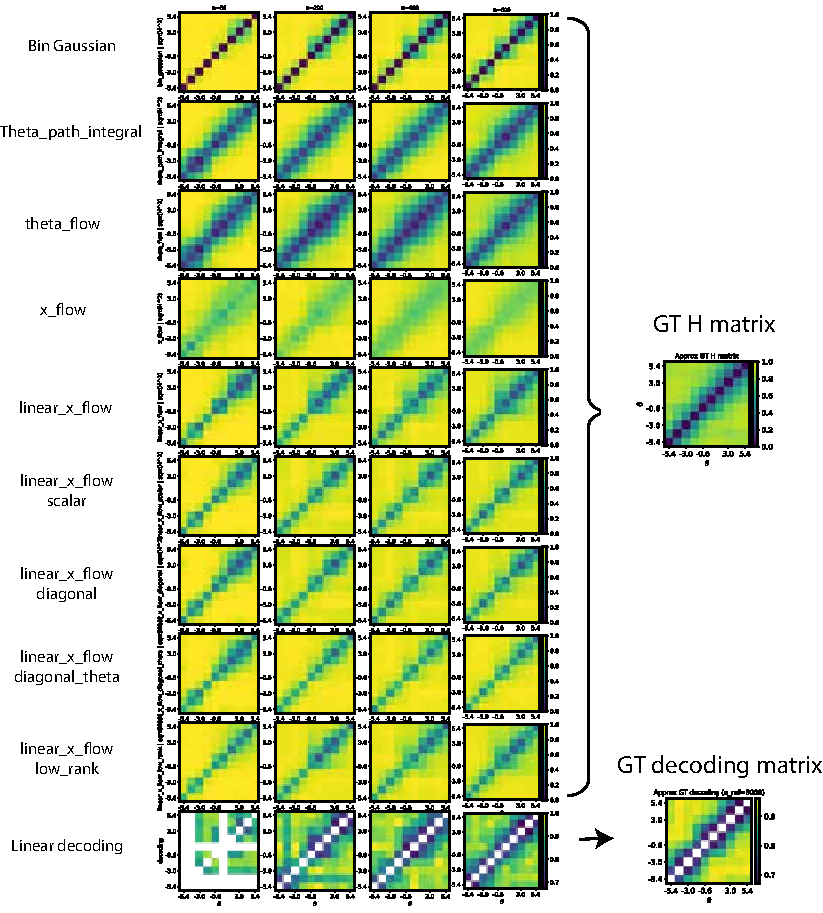
\includegraphics[width=\linewidth]{notes/figures/2026-04-30-linear-flow-matching/linear_flow_matching_si_fig1.pdf}
  \caption{%
  \textbf{Supplementary Figure 1.}
  Full matrix grids for the non-periodic setting at sample sizes $n\in\{80,200,400,600\}$.
  Rows: bin Gaussian, theta path integral, theta flow, $x$ flow, linear $x$ flow and its structured variants (scalar, diagonal, diagonal-in-$\theta$, low rank), and linear decoding.
  The first nine rows compare estimated $\sqrt{H^2}$ matrices to an approximate ground-truth $H$ matrix (right); the bottom row compares decoding accuracy matrices to an approximate ground-truth decoding reference ($n_{\mathrm{ref}}=3000$).%
  }
  \label{fig:linear-fm-si-1}
\end{figure}

\begin{figure}[!htbp]
  \centering
  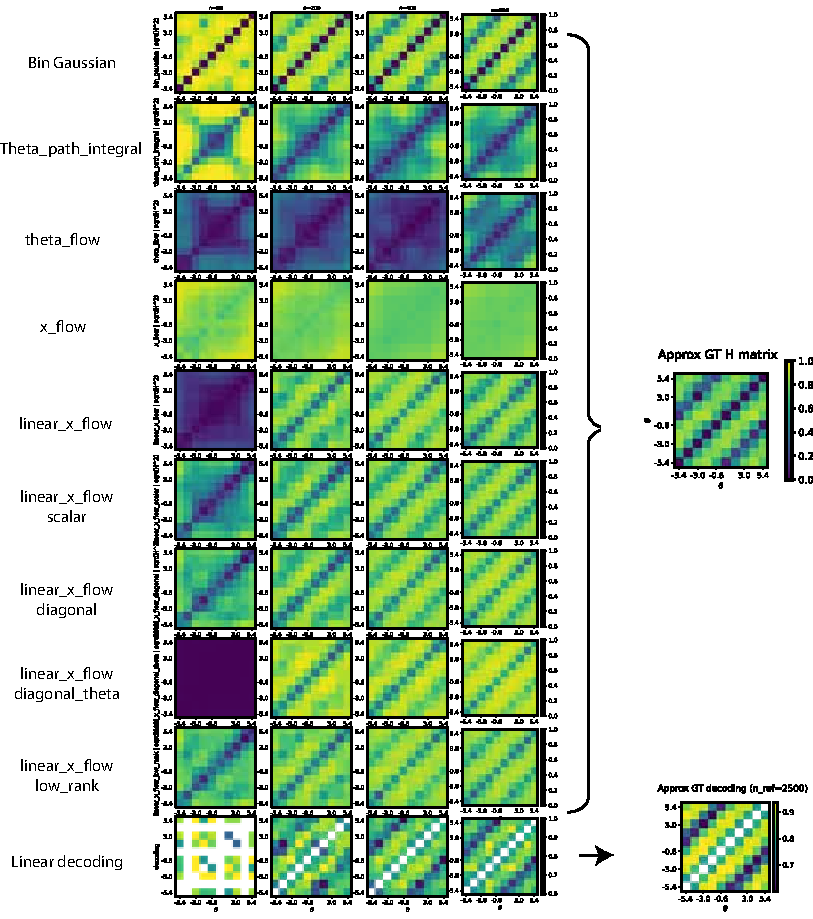
\includegraphics[width=\linewidth]{notes/figures/2026-04-30-linear-flow-matching/linear_flow_matching_si_fig2.pdf}
  \caption{%
  \textbf{Supplementary Figure 2.}
  Same layout as Supplementary Figure~\ref{fig:linear-fm-si-1} for the periodic high-dimensional setting.
  }
  \label{fig:linear-fm-si-2}
\end{figure}
